\section{eo\-Gnuplot Class Reference}
\label{classeo_gnuplot}\index{eoGnuplot@{eoGnuplot}}
Base class for calls to gnuplot.  


{\tt \#include $<$eo\-Gnuplot.h$>$}

Inheritance diagram for eo\-Gnuplot::\begin{figure}[H]
\begin{center}
\leavevmode
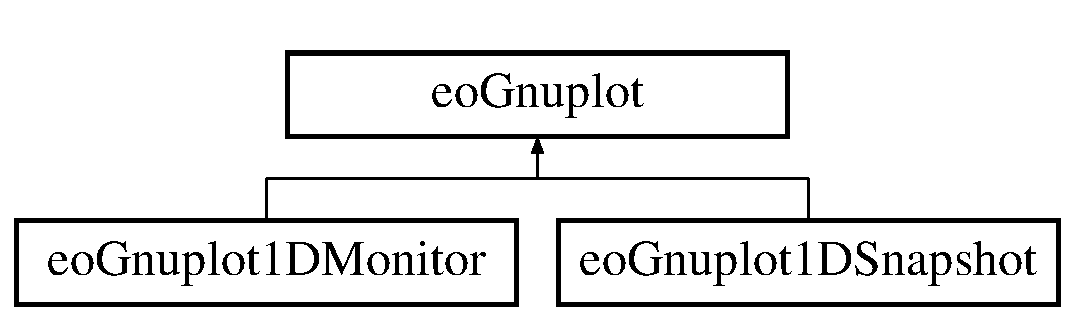
\includegraphics[height=2cm]{classeo_gnuplot}
\end{center}
\end{figure}
\subsection*{Public Member Functions}
\begin{CompactItemize}
\item 
{\bf eo\-Gnuplot} (std::string \_\-title, std::string \_\-extra=std::string(\char`\"{}\char`\"{}))
\begin{CompactList}\small\item\em Open pipe to Gnuplot. \item\end{CompactList}\item 
virtual {\bf $\sim$eo\-Gnuplot} ()
\begin{CompactList}\small\item\em Destructor. \item\end{CompactList}\item 
virtual std::string {\bf class\-Name} () const \label{classeo_gnuplot_a2}

\begin{CompactList}\small\item\em Class name. \item\end{CompactList}\item 
void {\bf gnuplot\-Command} (const char $\ast$\_\-command)\label{classeo_gnuplot_a3}

\begin{CompactList}\small\item\em Send command to gnuplot. \item\end{CompactList}\item 
void {\bf gnuplot\-Command} (std::string \_\-command)
\begin{CompactList}\small\item\em Send command to gnuplot. \item\end{CompactList}\end{CompactItemize}
\subsection*{Protected Member Functions}
\begin{CompactItemize}
\item 
void {\bf init\-Gnu\-Plot} (std::string \_\-title, std::string \_\-extra)
\begin{CompactList}\small\item\em Initialize gnuplot. \item\end{CompactList}\end{CompactItemize}
\subsection*{Protected Attributes}
\begin{CompactItemize}
\item 
bool {\bf first\-Time}\label{classeo_gnuplot_p0}

\begin{CompactList}\small\item\em The stats might be unknown in Ctor. \item\end{CompactList}\item 
PCom $\ast$ {\bf gp\-Com}\label{classeo_gnuplot_p1}

\begin{CompactList}\small\item\em Communication with gnuplot OK. \item\end{CompactList}\end{CompactItemize}
\subsection*{Static Protected Attributes}
\begin{CompactItemize}
\item 
unsigned {\bf num\-Window} = 0\label{classeo_gnuplot_t0}

\begin{CompactList}\small\item\em Internal counter for gnuplot windows. \item\end{CompactList}\end{CompactItemize}


\subsection{Detailed Description}
Base class for calls to gnuplot. 

This class is the abstract class that will be used by further gnuplot calls to plots what is already written by some {\bf eo\-Monitor}{\rm (p.\,\pageref{classeo_monitor})} into a file

\begin{Desc}
\item[Author:]Marc Schoenauer \end{Desc}
\begin{Desc}
\item[Version:]0.0 (2001) \end{Desc}




Definition at line 38 of file eo\-Gnuplot.h.

\subsection{Constructor \& Destructor Documentation}
\index{eoGnuplot@{eo\-Gnuplot}!eoGnuplot@{eoGnuplot}}
\index{eoGnuplot@{eoGnuplot}!eoGnuplot@{eo\-Gnuplot}}
\subsubsection{\setlength{\rightskip}{0pt plus 5cm}eo\-Gnuplot::eo\-Gnuplot (std::string {\em \_\-title}, std::string {\em \_\-extra} = {\tt std::string(\char`\"{}\char`\"{})})}\label{classeo_gnuplot_a0}


Open pipe to Gnuplot. 

\begin{Desc}
\item[Parameters:]
\begin{description}
\item[{\em \_\-title}]Title for gnuplot window. \item[{\em \_\-extra}]Extra parameters to gnuplot (default $<$none$>$). \end{description}
\end{Desc}


Definition at line 37 of file eo\-Gnuplot.cpp.

References init\-Gnu\-Plot().\index{eoGnuplot@{eo\-Gnuplot}!~eoGnuplot@{$\sim$eoGnuplot}}
\index{~eoGnuplot@{$\sim$eoGnuplot}!eoGnuplot@{eo\-Gnuplot}}
\subsubsection{\setlength{\rightskip}{0pt plus 5cm}eo\-Gnuplot::$\sim${\bf eo\-Gnuplot} ()\hspace{0.3cm}{\tt  [virtual]}}\label{classeo_gnuplot_a1}


Destructor. 

Close the gnuplot windows if pipe was correctly opened 

Definition at line 45 of file eo\-Gnuplot.cpp.

References gp\-Com.

\subsection{Member Function Documentation}
\index{eoGnuplot@{eo\-Gnuplot}!gnuplotCommand@{gnuplotCommand}}
\index{gnuplotCommand@{gnuplotCommand}!eoGnuplot@{eo\-Gnuplot}}
\subsubsection{\setlength{\rightskip}{0pt plus 5cm}void eo\-Gnuplot::gnuplot\-Command (std::string {\em \_\-command})\hspace{0.3cm}{\tt  [inline]}}\label{classeo_gnuplot_a4}


Send command to gnuplot. 

This is an overloaded member function, provided for convenience. It differs from the above function only in what argument(s) it accepts. 

Definition at line 66 of file eo\-Gnuplot.h.\index{eoGnuplot@{eo\-Gnuplot}!initGnuPlot@{initGnuPlot}}
\index{initGnuPlot@{initGnuPlot}!eoGnuplot@{eo\-Gnuplot}}
\subsubsection{\setlength{\rightskip}{0pt plus 5cm}void eo\-Gnuplot::init\-Gnu\-Plot (std::string {\em \_\-title}, std::string {\em \_\-extra})\hspace{0.3cm}{\tt  [protected]}}\label{classeo_gnuplot_b0}


Initialize gnuplot. 

\begin{Desc}
\item[Parameters:]
\begin{description}
\item[{\em \_\-title}]Title for gnuplot window. \item[{\em \_\-extra}]Extra parameters to gnuplot. \end{description}
\end{Desc}


Definition at line 70 of file eo\-Gnuplot.cpp.

References gp\-Com, and num\-Window.

Referenced by eo\-Gnuplot().

The documentation for this class was generated from the following files:\begin{CompactItemize}
\item 
eo\-Gnuplot.h\item 
eo\-Gnuplot.cpp\end{CompactItemize}
